% Created by tikzDevice version 0.12.3.1 on 2021-08-27 11:08:28
% !TEX encoding = UTF-8 Unicode
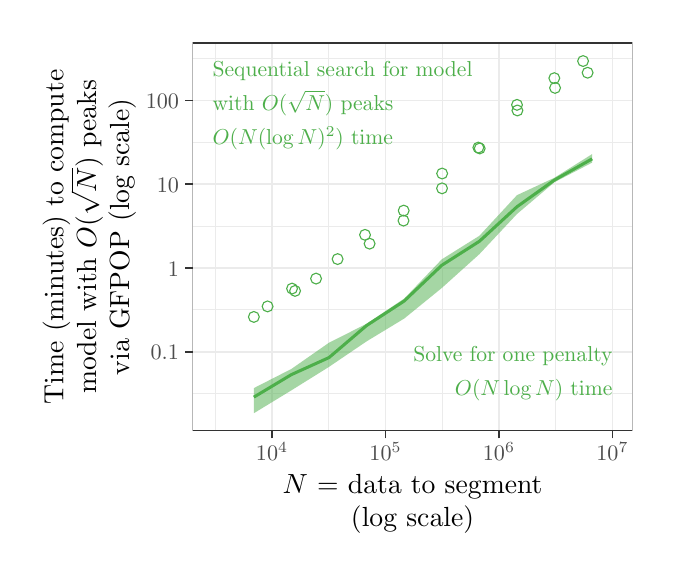
\begin{tikzpicture}[x=1pt,y=1pt]
\definecolor{fillColor}{RGB}{255,255,255}
\path[use as bounding box,fill=fillColor,fill opacity=0.00] (0,0) rectangle (224.04,187.90);
\begin{scope}
\path[clip] (  0.00,  0.00) rectangle (224.04,187.90);
\definecolor{drawColor}{RGB}{255,255,255}
\definecolor{fillColor}{RGB}{255,255,255}

\path[draw=drawColor,line width= 0.6pt,line join=round,line cap=round,fill=fillColor] ( -0.00,  0.00) rectangle (224.04,187.90);
\end{scope}
\begin{scope}
\path[clip] ( 59.62, 42.21) rectangle (218.54,182.40);
\definecolor{fillColor}{RGB}{255,255,255}

\path[fill=fillColor] ( 59.62, 42.21) rectangle (218.54,182.40);
\definecolor{drawColor}{gray}{0.92}

\path[draw=drawColor,line width= 0.3pt,line join=round] ( 59.62, 55.66) --
	(218.54, 55.66);

\path[draw=drawColor,line width= 0.3pt,line join=round] ( 59.62, 85.93) --
	(218.54, 85.93);

\path[draw=drawColor,line width= 0.3pt,line join=round] ( 59.62,116.19) --
	(218.54,116.19);

\path[draw=drawColor,line width= 0.3pt,line join=round] ( 59.62,146.46) --
	(218.54,146.46);

\path[draw=drawColor,line width= 0.3pt,line join=round] ( 59.62,176.72) --
	(218.54,176.72);

\path[draw=drawColor,line width= 0.3pt,line join=round] ( 67.78, 42.21) --
	( 67.78,182.40);

\path[draw=drawColor,line width= 0.3pt,line join=round] (108.79, 42.21) --
	(108.79,182.40);

\path[draw=drawColor,line width= 0.3pt,line join=round] (149.80, 42.21) --
	(149.80,182.40);

\path[draw=drawColor,line width= 0.3pt,line join=round] (190.81, 42.21) --
	(190.81,182.40);

\path[draw=drawColor,line width= 0.6pt,line join=round] ( 59.62, 70.79) --
	(218.54, 70.79);

\path[draw=drawColor,line width= 0.6pt,line join=round] ( 59.62,101.06) --
	(218.54,101.06);

\path[draw=drawColor,line width= 0.6pt,line join=round] ( 59.62,131.32) --
	(218.54,131.32);

\path[draw=drawColor,line width= 0.6pt,line join=round] ( 59.62,161.59) --
	(218.54,161.59);

\path[draw=drawColor,line width= 0.6pt,line join=round] ( 88.28, 42.21) --
	( 88.28,182.40);

\path[draw=drawColor,line width= 0.6pt,line join=round] (129.29, 42.21) --
	(129.29,182.40);

\path[draw=drawColor,line width= 0.6pt,line join=round] (170.30, 42.21) --
	(170.30,182.40);

\path[draw=drawColor,line width= 0.6pt,line join=round] (211.31, 42.21) --
	(211.31,182.40);
\definecolor{drawColor}{RGB}{77,175,74}

\node[text=drawColor,anchor=base west,inner sep=0pt, outer sep=0pt, scale=  0.78] at ( 66.84,170.29) {Sequential search for model};

\node[text=drawColor,anchor=base west,inner sep=0pt, outer sep=0pt, scale=  0.78] at ( 66.84,158.00) {with $O(\sqrt N)$ peaks};

\node[text=drawColor,anchor=base west,inner sep=0pt, outer sep=0pt, scale=  0.78] at ( 66.84,145.71) {$O(N(\log N)^2)$ time};

\node[text=drawColor,anchor=base east,inner sep=0pt, outer sep=0pt, scale=  0.78] at (211.31, 67.26) {Solve for one penalty};

\node[text=drawColor,anchor=base east,inner sep=0pt, outer sep=0pt, scale=  0.78] at (211.31, 54.97) {$O(N \log N)$ time};
\definecolor{fillColor}{RGB}{77,175,74}

\path[fill=fillColor,fill opacity=0.50] ( 81.73, 57.66) --
	( 95.31, 64.59) --
	(108.89, 74.06) --
	(122.47, 80.91) --
	(136.06, 90.01) --
	(149.64,104.19) --
	(163.22,112.69) --
	(176.80,127.37) --
	(190.38,133.69) --
	(203.97,142.22) --
	(203.97,139.13) --
	(190.38,132.07) --
	(176.80,120.56) --
	(163.22,106.05) --
	(149.64, 93.83) --
	(136.06, 82.79) --
	(122.47, 74.55) --
	(108.89, 65.34) --
	( 95.31, 56.86) --
	( 81.73, 48.58) --
	cycle;

\path[] ( 81.73, 57.66) --
	( 95.31, 64.59) --
	(108.89, 74.06) --
	(122.47, 80.91) --
	(136.06, 90.01) --
	(149.64,104.19) --
	(163.22,112.69) --
	(176.80,127.37) --
	(190.38,133.69) --
	(203.97,142.22);

\path[] (203.97,139.13) --
	(190.38,132.07) --
	(176.80,120.56) --
	(163.22,106.05) --
	(149.64, 93.83) --
	(136.06, 82.79) --
	(122.47, 74.55) --
	(108.89, 65.34) --
	( 95.31, 56.86) --
	( 81.73, 48.58);

\path[draw=drawColor,line width= 1.1pt,line join=round] ( 81.73, 54.40) --
	( 95.31, 62.54) --
	(108.89, 68.69) --
	(122.47, 80.27) --
	(136.06, 89.12) --
	(149.64,102.04) --
	(163.22,110.70) --
	(176.80,123.18) --
	(190.38,132.86) --
	(203.97,140.50);

\path[draw=drawColor,line width= 0.4pt,line join=round,line cap=round] ( 81.73, 83.38) circle (  1.96);

\path[draw=drawColor,line width= 0.4pt,line join=round,line cap=round] ( 86.69, 87.18) circle (  1.96);

\path[draw=drawColor,line width= 0.4pt,line join=round,line cap=round] ( 95.53, 93.62) circle (  1.96);

\path[draw=drawColor,line width= 0.4pt,line join=round,line cap=round] ( 96.62, 92.78) circle (  1.96);

\path[draw=drawColor,line width= 0.4pt,line join=round,line cap=round] (104.21, 97.23) circle (  1.96);

\path[draw=drawColor,line width= 0.4pt,line join=round,line cap=round] (111.99,104.28) circle (  1.96);

\path[draw=drawColor,line width= 0.4pt,line join=round,line cap=round] (121.90,113.04) circle (  1.96);

\path[draw=drawColor,line width= 0.4pt,line join=round,line cap=round] (123.55,109.85) circle (  1.96);

\path[draw=drawColor,line width= 0.4pt,line join=round,line cap=round] (135.80,118.18) circle (  1.96);

\path[draw=drawColor,line width= 0.4pt,line join=round,line cap=round] (135.87,121.80) circle (  1.96);

\path[draw=drawColor,line width= 0.4pt,line join=round,line cap=round] (149.73,129.84) circle (  1.96);

\path[draw=drawColor,line width= 0.4pt,line join=round,line cap=round] (149.77,135.20) circle (  1.96);

\path[draw=drawColor,line width= 0.4pt,line join=round,line cap=round] (162.85,144.58) circle (  1.96);

\path[draw=drawColor,line width= 0.4pt,line join=round,line cap=round] (163.34,144.25) circle (  1.96);

\path[draw=drawColor,line width= 0.4pt,line join=round,line cap=round] (176.82,160.01) circle (  1.96);

\path[draw=drawColor,line width= 0.4pt,line join=round,line cap=round] (176.97,157.98) circle (  1.96);

\path[draw=drawColor,line width= 0.4pt,line join=round,line cap=round] (190.30,169.66) circle (  1.96);

\path[draw=drawColor,line width= 0.4pt,line join=round,line cap=round] (190.57,166.13) circle (  1.96);

\path[draw=drawColor,line width= 0.4pt,line join=round,line cap=round] (200.69,175.84) circle (  1.96);

\path[draw=drawColor,line width= 0.4pt,line join=round,line cap=round] (202.33,171.62) circle (  1.96);
\definecolor{drawColor}{gray}{0.20}

\path[draw=drawColor,line width= 0.6pt,line join=round,line cap=round] ( 59.62, 42.21) rectangle (218.54,182.40);
\end{scope}
\begin{scope}
\path[clip] (  0.00,  0.00) rectangle (224.04,187.90);
\definecolor{drawColor}{gray}{0.30}

\node[text=drawColor,anchor=base east,inner sep=0pt, outer sep=0pt, scale=  0.80] at ( 54.67, 67.84) {0.1};

\node[text=drawColor,anchor=base east,inner sep=0pt, outer sep=0pt, scale=  0.80] at ( 54.67, 98.10) {1};

\node[text=drawColor,anchor=base east,inner sep=0pt, outer sep=0pt, scale=  0.80] at ( 54.67,128.37) {10};

\node[text=drawColor,anchor=base east,inner sep=0pt, outer sep=0pt, scale=  0.80] at ( 54.67,158.63) {100};
\end{scope}
\begin{scope}
\path[clip] (  0.00,  0.00) rectangle (224.04,187.90);
\definecolor{drawColor}{gray}{0.20}

\path[draw=drawColor,line width= 0.6pt,line join=round] ( 56.87, 70.79) --
	( 59.62, 70.79);

\path[draw=drawColor,line width= 0.6pt,line join=round] ( 56.87,101.06) --
	( 59.62,101.06);

\path[draw=drawColor,line width= 0.6pt,line join=round] ( 56.87,131.32) --
	( 59.62,131.32);

\path[draw=drawColor,line width= 0.6pt,line join=round] ( 56.87,161.59) --
	( 59.62,161.59);
\end{scope}
\begin{scope}
\path[clip] (  0.00,  0.00) rectangle (224.04,187.90);
\definecolor{drawColor}{gray}{0.20}

\path[draw=drawColor,line width= 0.6pt,line join=round] ( 88.28, 39.46) --
	( 88.28, 42.21);

\path[draw=drawColor,line width= 0.6pt,line join=round] (129.29, 39.46) --
	(129.29, 42.21);

\path[draw=drawColor,line width= 0.6pt,line join=round] (170.30, 39.46) --
	(170.30, 42.21);

\path[draw=drawColor,line width= 0.6pt,line join=round] (211.31, 39.46) --
	(211.31, 42.21);
\end{scope}
\begin{scope}
\path[clip] (  0.00,  0.00) rectangle (224.04,187.90);
\definecolor{drawColor}{gray}{0.30}

\node[text=drawColor,anchor=base,inner sep=0pt, outer sep=0pt, scale=  0.80] at ( 88.28, 31.34) {$10^4$};

\node[text=drawColor,anchor=base,inner sep=0pt, outer sep=0pt, scale=  0.80] at (129.29, 31.34) {$10^5$};

\node[text=drawColor,anchor=base,inner sep=0pt, outer sep=0pt, scale=  0.80] at (170.30, 31.34) {$10^6$};

\node[text=drawColor,anchor=base,inner sep=0pt, outer sep=0pt, scale=  0.80] at (211.31, 31.34) {$10^7$};
\end{scope}
\begin{scope}
\path[clip] (  0.00,  0.00) rectangle (224.04,187.90);
\definecolor{drawColor}{RGB}{0,0,0}

\node[text=drawColor,anchor=base,inner sep=0pt, outer sep=0pt, scale=  1.00] at (139.08, 19.50) {$N$ = data to segment};

\node[text=drawColor,anchor=base,inner sep=0pt, outer sep=0pt, scale=  1.00] at (139.08,  7.62) {(log scale)};
\end{scope}
\begin{scope}
\path[clip] (  0.00,  0.00) rectangle (224.04,187.90);
\definecolor{drawColor}{RGB}{0,0,0}

\node[text=drawColor,rotate= 90.00,anchor=base,inner sep=0pt, outer sep=0pt, scale=  1.00] at ( 12.89,112.30) {Time (minutes) to compute};

\node[text=drawColor,rotate= 90.00,anchor=base,inner sep=0pt, outer sep=0pt, scale=  1.00] at ( 24.77,112.30) {     model with $O(\sqrt N)$ peaks};

\node[text=drawColor,rotate= 90.00,anchor=base,inner sep=0pt, outer sep=0pt, scale=  1.00] at ( 36.65,112.30) {     via GFPOP (log scale)};
\end{scope}
\end{tikzpicture}
